% =====================================================
\chapter{Literature Survey}
\label{chap:literature_survey}

This chapter builds the theoretical foundation for the work presented in this thesis.
It traces the evolution of modern generative modelling from attention-based architectures such as Transformers~\cite{vaswani2017attention} and Vision Transformers~\cite{dosovitskiy2020vit} through generative frameworks like GANs~\cite{goodfellow2014gan} and VAEs~\cite{kingma2013autoencoding}, culminating in diffusion models that now dominate controllable image synthesis.
The discussion then explores conditioning mechanisms, adapters, and perceptual style descriptors --- CLIP~\cite{radford2021clip}, CSD~\cite{somepalli2024measuring}, IP-Adapter~\cite{ye2023ipadapterfidelityadapters} --- that make diffusion models both semantically and stylistically aware.
Subsequent sections cover frequency-domain operators, domain adaptation, optimization-guided diffusion, and physics-based atmospheric image formation.

% =====================================================
\section{Transformers: Attention-Based Sequence Modelling}
\label{sec:transformers}

Transformers~\cite{vaswani2017attention} revolutionised neural network design by discarding recurrence in favour of parallel attention.
Every element of a sequence can attend to every other, learning global context in a single step.
The self-attention mechanism is defined as:
\[
\mathrm{Attention}(Q,K,V)
=\mathrm{softmax}\!\Big(\frac{QK^\top}{\sqrt{d_k}}\Big)V, \qquad
Q=XW_Q,\;K=XW_K,\;V=XW_V.
\]
Residual connections and layer normalisation stabilise deep stacks~\cite{vaswani2017attention}, while positional encodings supply sequence order.
Transformers became the blueprint for multimodal systems such as CLIP~\cite{radford2021clip}, Stable Diffusion~\cite{rombach2022ldm}, and IP-Adapter~\cite{ye2023ipadapterfidelityadapters}, where attention serves as the communication channel between modalities.
In diffusion models, this principle governs how textual or visual prompts communicate with the U-Net~\cite{ronneberger2015unet} at each denoising step.

\begin{figure}[!htbp]
  \centering
  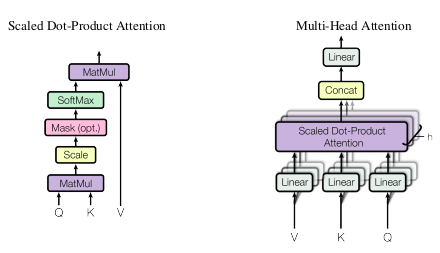
\includegraphics[width=0.75\linewidth]{images/transformer_attention.png}
  \caption{Self-attention pipeline: query--key similarity produces data-dependent mixing of values (adapted from Vaswani et al., 2017~\cite{vaswani2017attention}).}
  \label{fig:transformer_attention}
\end{figure}
\FloatBarrier

% =====================================================
\section{Vision Transformers (ViT)}
\label{sec:lit_vit}

The Vision Transformer (ViT)~\cite{dosovitskiy2020vit} treats an image as a sequence of non-overlapping $P{\times}P$ patches that act as tokens.
Each patch is linearly projected and combined with positional embeddings before passing through stacked transformer encoders.
A [CLS] token aggregates global information for classification.
ViT removes locality bias and allows any patch to attend to any other, thereby capturing long-range dependencies such as fog gradients or underwater scattering that are critical for environmental style modelling.

\begin{figure}[!htbp]
  \centering
  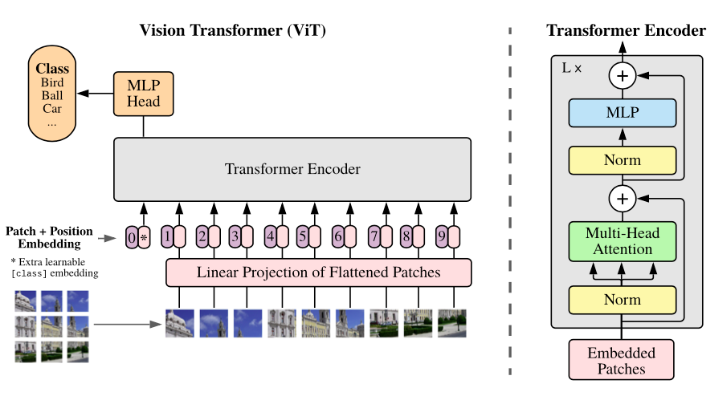
\includegraphics[width=0.75\linewidth]{images/vit_pipeline.png}
  \caption{ViT pipeline and Transformer Block (adapted from Dosovitskiy et al., 2021~\cite{dosovitskiy2020vit}).}
  \label{fig:vit_pipeline}
\end{figure}
\FloatBarrier

% =====================================================
\section{Adaptive Fourier Neural Operators (AFNO)}
\label{sec:afno}

Fourier Neural Operators (FNOs) are used for token mixing in the frequency domain.
Adaptive Fourier Neural Operators (AFNO)~\cite{guibas2021afno} extend FNOs by transforming feature representations to the spectral domain via the Fast Fourier Transform (FFT), which can efficiently model global interactions through operations in frequency space, rather than traditional self-attention mechanisms that are performed directly on spatial tokens.

\noindent The main idea behind AFNO is that many visual patterns are more compactly represented in the frequency domain.
Instead of manipulating individual spatial tokens, AFNO manipulates frequency coefficients to capture long-range dependencies with dramatically reduced computational complexity.
This property has made AFNO effective in large-scale vision tasks, image restoration, weather forecasting, and scientific machine learning applications.

\noindent Given an input feature representation $X \in \mathbb{R}^{H \times W \times C}$, AFNO first maps the feature map to the Fourier domain by a two-dimensional Fourier transform:
\begin{equation}
    \hat{X} = \mathcal{F}(X),
\end{equation}
where $\mathcal{F}(\cdot)$ is the Fourier transform operation.
The transformed coefficients are then spectrally filtered --- with hard-thresholding and soft-shrinkage enforcing sparsity across frequency modes --- and the representation is transformed back to the spatial domain with the inverse Fourier transform.

\noindent One key advantage of AFNO is the ability to model the global structure of images via frequency-space interactions.
Since atmospheric degradations such as haze, fog, smoke, and snowfall tend to preserve coarse scene structure while suppressing high-frequency image information, frequency-domain processing provides a natural mechanism for modelling such degradations.
In this thesis, AFNO adapters are inserted into frozen ViT backbones to selectively modulate frequency bands affected by atmospheric corruption without disturbing the pretrained representations.

\begin{figure}[!htbp]
  \centering
  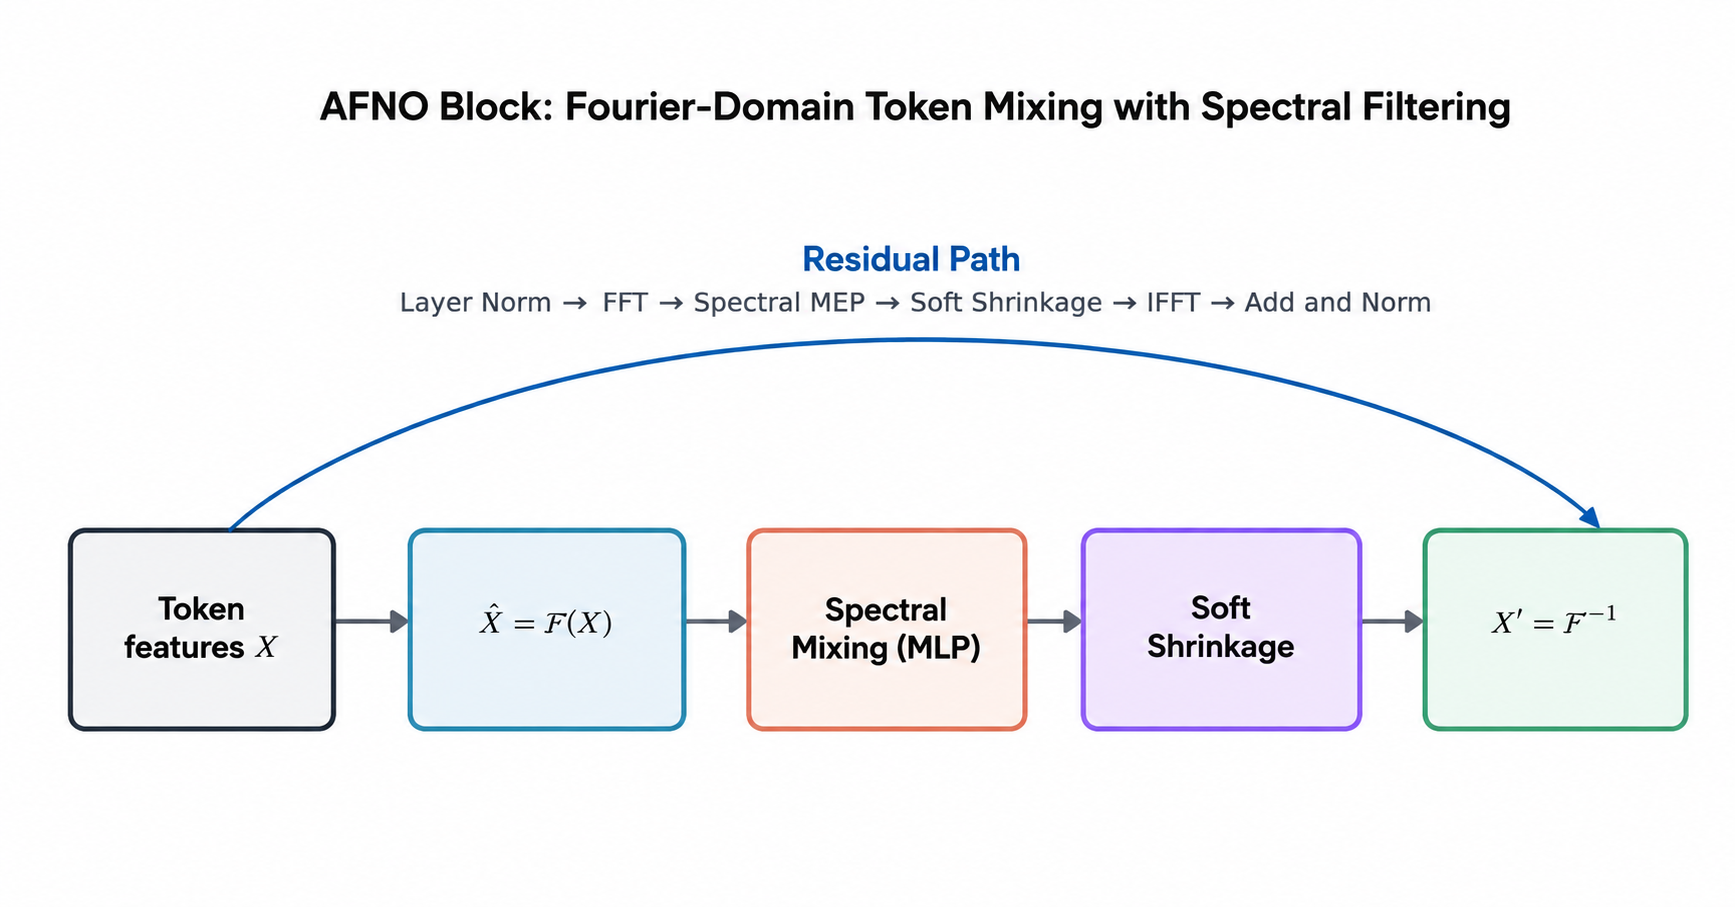
\includegraphics[width=0.92\linewidth]{images/figure_2.3.png}
  \caption{Overview of the Adaptive Fourier Neural Operator (AFNO) block with Fourier-domain token mixing and spectral filtering (adapted from Guibas et al., 2022~\cite{guibas2021afno}).}
  \label{fig:afno}
\end{figure}
\FloatBarrier

\noindent Recent works have shown the effectiveness of AFNO-based architectures for handling large-scale visual transformations and distribution shifts.
The power of AFNO for selective spectral representation manipulation is of particular importance for adaptation under strong atmospheric degradations, where frequency properties differ substantially from those of clean images.

% =====================================================
\section{Generative Adversarial Networks (GANs)}
\label{sec:gans}

\textbf{Generative Adversarial Networks (GANs)}~\cite{goodfellow2014gan} were the first to produce high-fidelity synthetic images.
They train a Generator $G$ and Discriminator $D$ in an adversarial loop:
\[
\min_G \max_D
\mathbb{E}_{x\sim p_\text{data}}[\log D(x)]
+\mathbb{E}_{z\sim p_z}[\log(1-D(G(z)))].
\]
GANs introduced sampling from a learned distribution rather than memorising examples, but adversarial training often causes instability and mode collapse.
Variants such as WGAN~\cite{arjovsky2017wassersteingan} and StyleGAN~\cite{karras2019stylegan} improved visual realism; however, they lacked semantic control and physical interpretability.
The PatchGAN discriminator from Isola et al.~\cite{isola2017image2image} classifies $N\times N$ image patches rather than the full image, and is reused in KDA-Net's haze-authenticator sub-network (Chapter~\ref{chap:phase2_pipeline}).

\begin{figure}[!htbp]
  \centering
  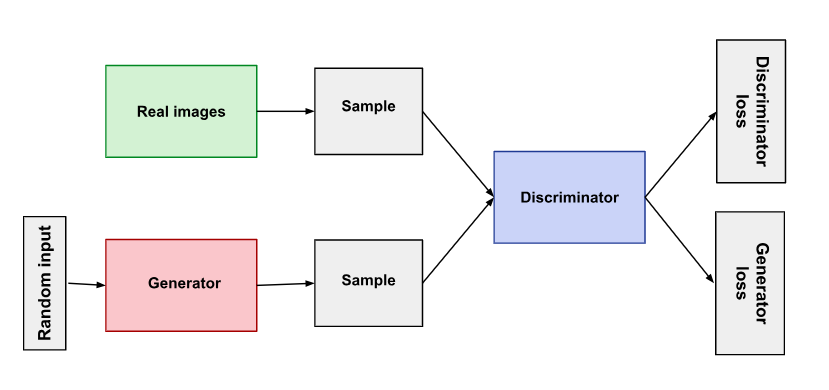
\includegraphics[width=0.72\linewidth]{images/gan_architecture.png}
  \caption{GAN architecture: generator--discriminator adversarial training loop (adapted from Foster, 2023~\cite{foster2023generativedeeplearning}).}
  \label{fig:gan_architecture}
\end{figure}
\FloatBarrier

% =====================================================
\section{Variational Autoencoders (VAEs)}
\label{sec:vaes}

VAEs~\cite{kingma2013autoencoding} model data generation via a continuous latent variable $z$.
They maximise the Evidence Lower Bound (ELBO):
\[
\log p_\theta(x) \ge
\mathbb{E}_{q_\phi(z|x)}[\log p_\theta(x|z)]
- \mathrm{KL}\!\big(q_\phi(z|x)\|p(z)\big),
\quad
z = \mu_\phi(x) + \sigma_\phi(x)\odot\epsilon.
\]
VAEs yield smooth, interpretable latent manifolds enabling continuous interpolation between images.
Although outputs can appear slightly blurred, VAEs provide stability and differentiable latent sampling --- properties later exploited in Latent Diffusion Models (LDMs)~\cite{rombach2022ldm}.

\begin{figure}[!htbp]
  \centering
  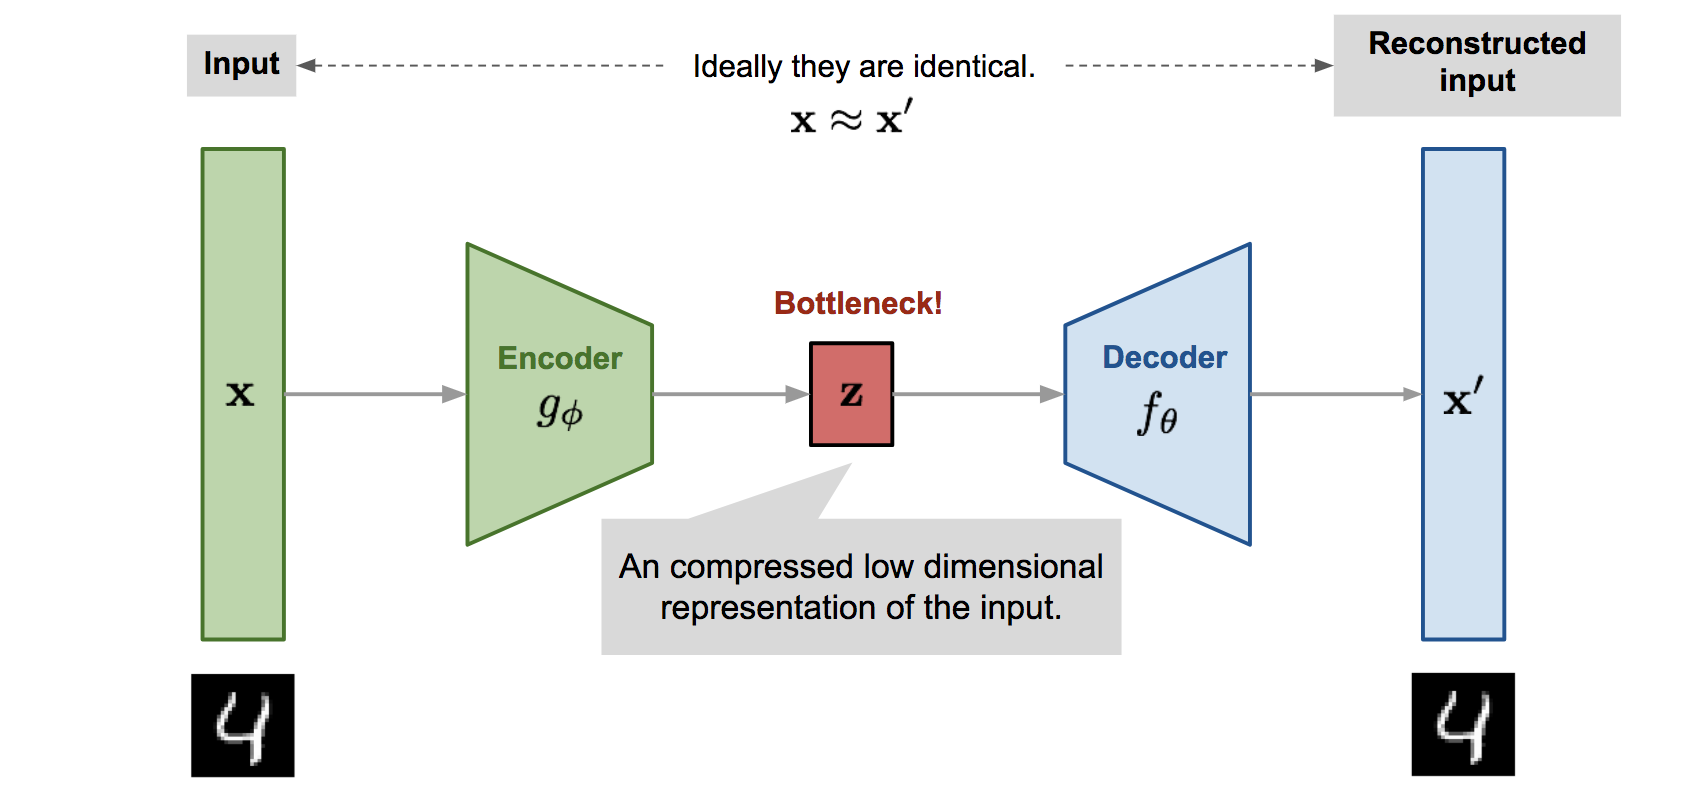
\includegraphics[width=0.75\linewidth]{images/vae_architecture.png}
  \caption{Variational Autoencoder: encoder--decoder with reparameterisation trick (adapted from Foster, 2023~\cite{foster2023generativedeeplearning}).}
  \label{fig:vae_architecture}
\end{figure}
\FloatBarrier

% =====================================================
\section{U-Net Backbone for Diffusion}
\label{sec:lit_unet}

U-Net~\cite{ronneberger2015unet} provides hierarchical feature extraction through an encoder--decoder architecture with skip connections that preserve fine detail.
Diffusion models augment U-Net with \textbf{time-step embeddings} (representing noise level) and \textbf{cross-attention layers} (for text or image conditions), forming the structural engine of modern denoising diffusion.
The encoder progressively downsamples the noisy image into coarse latent features capturing global semantics, while the decoder reconstructs spatial details through upsampling.
Skip connections ensure that high-frequency information from the encoder is passed directly to the corresponding decoder stage.
Time-step embeddings allow the model to adjust its denoising strength dynamically --- focusing on coarse structure during early steps and fine details in later stages.
Cross-attention integrates contextual guidance, enabling the model to align visual content with prompts, reference styles, or other conditioning inputs.

\begin{figure}[!h]
  \centering
  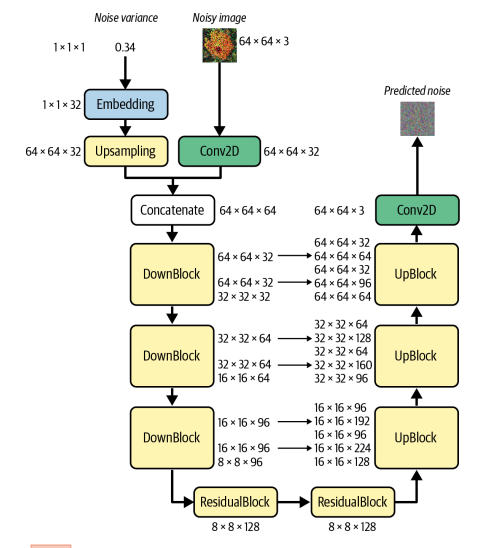
\includegraphics[width=0.60\linewidth]{images/unet_architecture.png}
  \caption{Diffusion U-Net: encoder--decoder with skip connections, time-step embeddings, and cross-attention (adapted from Foster, 2023~\cite{foster2023generativedeeplearning}).}
  \label{fig:unet_architecture}
\end{figure}
\FloatBarrier

% =====================================================
\section{Diffusion Models}
\label{sec:diffusion_models}

Diffusion models~\cite{ho2020ddpm} constitute a family of generative models that gradually convert pure noise into structured data through a learned denoising process, interpreting image generation as the reversal of a stochastic diffusion process.

\subsection*{Forward Process}

The forward process progressively destroys image structure by adding Gaussian noise over $T$ timesteps according to a variance schedule $\{\beta_t\}_{t=1}^T$:
\[
q(x_t|x_{t-1})=\mathcal{N}\big(\sqrt{1-\beta_t}\,x_{t-1},\,\beta_t I\big), \qquad
x_t = \sqrt{\bar{\alpha}_t}\,x_0 + \sqrt{1-\bar{\alpha}_t}\,\epsilon,
\quad \bar{\alpha}_t = \prod_{i=1}^t (1-\beta_i).
\]
As $t\!\to\!T$, $x_T$ approaches pure noise.

\begin{figure}[!htbp]
  \centering
  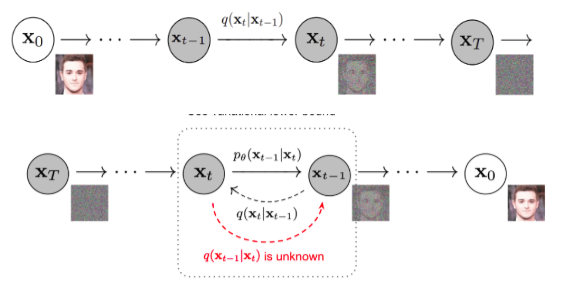
\includegraphics[width=0.75\linewidth]{images/ddpm_forward_reverse.png}
  \caption{Forward and reverse diffusion: corruption by Gaussian noise and stepwise denoising (adapted from Foster, 2023~\cite{foster2023generativedeeplearning}).}
  \label{fig:diffusion_process}
\end{figure}
\FloatBarrier

\subsection*{Reverse Process}

A neural network $\epsilon_\theta(x_t,t)$ is trained to predict the noise at each timestep:
\[
p_\theta(x_{t-1}|x_t)
=\mathcal{N}\!\big(\mu_\theta(x_t,t),\,\sigma_t^2 I\big), \quad
\mathcal{L}_{\text{simple}}
=\mathbb{E}_{x_0,t,\epsilon}
\big[\|\epsilon-\epsilon_\theta(\sqrt{\bar{\alpha}_t}x_0+\sqrt{1-\bar{\alpha}_t}\epsilon,t)\|^2\big].
\]
At inference, the process begins from $x_T\!\sim\!\mathcal{N}(0,I)$ and iteratively denoises until $x_0$ emerges.
DDIM~\cite{song2021ddim} reformulates this as a non-Markovian process enabling deterministic sampling in 40--50 steps rather than 1000, and is the inference scheduler used throughout this work.

\subsection*{Conditional and Guided Diffusion}
\label{sec:conditional_diffusion}

An external classifier $p_\phi(y|x_t)$ can guide sampling by adjusting the predicted noise~\cite{dhariwal2021diffusion}:
\[
\tilde{\epsilon}_\theta(x_t,t|y)
=\epsilon_\theta(x_t,t)
- w\,\sigma_t\nabla_{x_t}\log p_\phi(y|x_t).
\]
Modern diffusion integrates conditioning directly inside the U-Net via cross-attention, with $(K,V)$ from conditioning encoders (text or style) and $Q$ from U-Net activations.

\subsection*{Latent Diffusion and Stable Diffusion}
\label{sec:ldm_stable}

Latent Diffusion Models (LDMs)~\cite{rombach2022ldm} perform diffusion in the latent space of a pretrained VAE, drastically reducing computation.
SDXL~\cite{podell2023sdxlimprovinglatentdiffusion} extends this with dual-encoder text conditioning (CLIP ViT-L/14 + OpenCLIP ViT-bigG) at $1024\times1024$ native resolution.
It is the generative backbone for all experiments in this work.

\begin{figure}[!htbp]
  \centering
  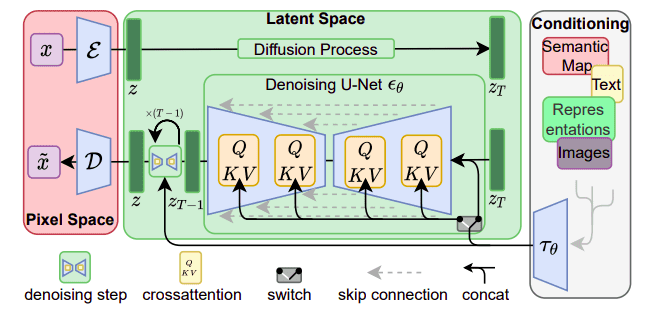
\includegraphics[width=0.7\linewidth]{images/stable_diffusion_architecture.png}
  \caption{Stable Diffusion: text-conditioned latent denoising within a VAE encoder--decoder pipeline (adapted from Foster, 2023~\cite{foster2023generativedeeplearning}).}
  \label{fig:stable_diffusion}
\end{figure}
\FloatBarrier

% =====================================================
\section{CLIP Encoders and Vision-Language Models}
\label{sec:clip}

Vision-language models have become a powerful paradigm for learning generalised visual representations with large-scale multimodal pretraining.
Instead of depending on manually annotated class labels, these models learn aligned representations between images and natural language descriptions that can be effectively transferred to a wide range of downstream tasks.

\noindent Contrastive Language-Image Pretraining (CLIP)~\cite{radford2021clip} is one of the most influential vision-language models.
CLIP has two independent encoders: an image encoder and a text encoder.
During training, images and text are projected into a common embedding space using a contrastive objective that pulls similar pairs together and pushes apart dissimilar pairs.

\noindent Let $I$ denote an image and $T$ its corresponding text description.
CLIP learns image and text embeddings:
\begin{equation}
    z_I = f_I(I), \qquad z_T = f_T(T),
\end{equation}
where $f_I$ and $f_T$ are the image and text encoders respectively.
The cosine similarity between the embeddings is:
\begin{equation}
    s(I,T) = \frac{z_I \cdot z_T}{\|z_I\|\,\|z_T\|}.
\end{equation}
This formulation allows zero-shot classification by matching image embeddings with textual descriptions of candidate categories.
Training uses the InfoNCE loss:
\[
\mathcal{L}_{\text{CLIP}}
=-\frac{1}{N}\sum_{i=1}^N
\Big[
\log\frac{e^{s(I_i,T_i)/\tau}}{\sum_j e^{s(I_i,T_j)/\tau}}
+\log\frac{e^{s(I_i,T_i)/\tau}}{\sum_j e^{s(I_j,T_i)/\tau}}
\Big].
\]

\begin{figure}[!htbp]
  \centering
  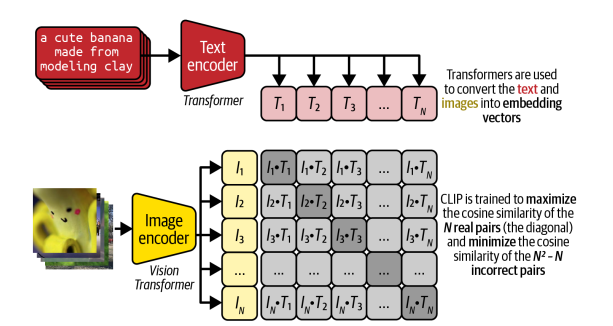
\includegraphics[width=0.65\linewidth]{images/clip_contrastive.png}
  \caption{CLIP architecture with separate image and text encoders trained with contrastive learning (adapted from Foster, 2023~\cite{foster2023generativedeeplearning}).}
  \label{fig:clip_contrastive}
\end{figure}
\FloatBarrier

\noindent CLIP's large-scale pretraining paradigm has proven remarkably robust and transferable to a wide range of visual tasks.
However, it is well established that severe environmental degradations can still impact the quality of its representations, motivating the adaptation strategies developed in this thesis.

% =====================================================
\section{Contrastive Style Descriptors (CSD)}
\label{sec:csd}

The success of large-scale vision-language models has generated growing interest in learning representations that separate semantic content from visual style.
Semantic representations describe the objects and structure of an image, while style representations describe attributes such as texture, colour distribution, illumination, atmospheric conditions, and artistic characteristics.
Properly disentangling these factors is of great value for controllable image synthesis and style-guided generation.

\noindent Conventional style transfer methods generally depend on low-level feature statistics extracted from convolutional neural networks.
Such representations capture texture information but often fail to provide robust semantic understanding of style across different image domains.
Recent works have therefore explored contrastive learning approaches for learning more sophisticated style representations directly from large-scale visual datasets.

\noindent Contrastive Style Descriptors (CSD)~\cite{somepalli2024measuring} offer a framework for learning disentangled representations of style and content via contrastive learning.
CSD builds upon frozen CLIP encoders, where different projection heads learn style-aware and content-aware representations while preserving the semantic knowledge learned in the CLIP feature space.

\noindent Given an image representation $z$ extracted from a pretrained CLIP encoder, CSD learns separate style and content mappings:
\begin{equation}
    z_s = f_s(z), \qquad z_c = f_c(z),
\end{equation}
where $f_s$ and $f_c$ are style and content projection functions respectively.
The goal is to have images with similar stylistic characteristics be close to each other in the style embedding space while being well separated from semantically different styles.
This is achieved using contrastive objectives that maximise agreement between positive style pairs and minimise similarity between negative pairs.
Similarity is computed as:
\[
\mathrm{Sim}(x_g, x_r) = \frac{z_g^\top z_r}{\|z_g\|\,\|z_r\|}.
\]


\noindent This results in style representations that semantically describe atmospheric characteristics such as haze, snow, smoke, and sandstorms.
Contrastive style descriptors are more robust and better match human perception of environmental appearance than traditional texture-statistics-based style representations.

\noindent The ability to measure stylistic similarity in a learned embedding space enables new forms of controllable image generation and style-guided diffusion.
In particular, style descriptors can be employed as a guiding signal during the diffusion process, steering generated samples towards desired atmospheric characteristics while preserving scene structure.

\begin{figure}[htbp]
    \centering
    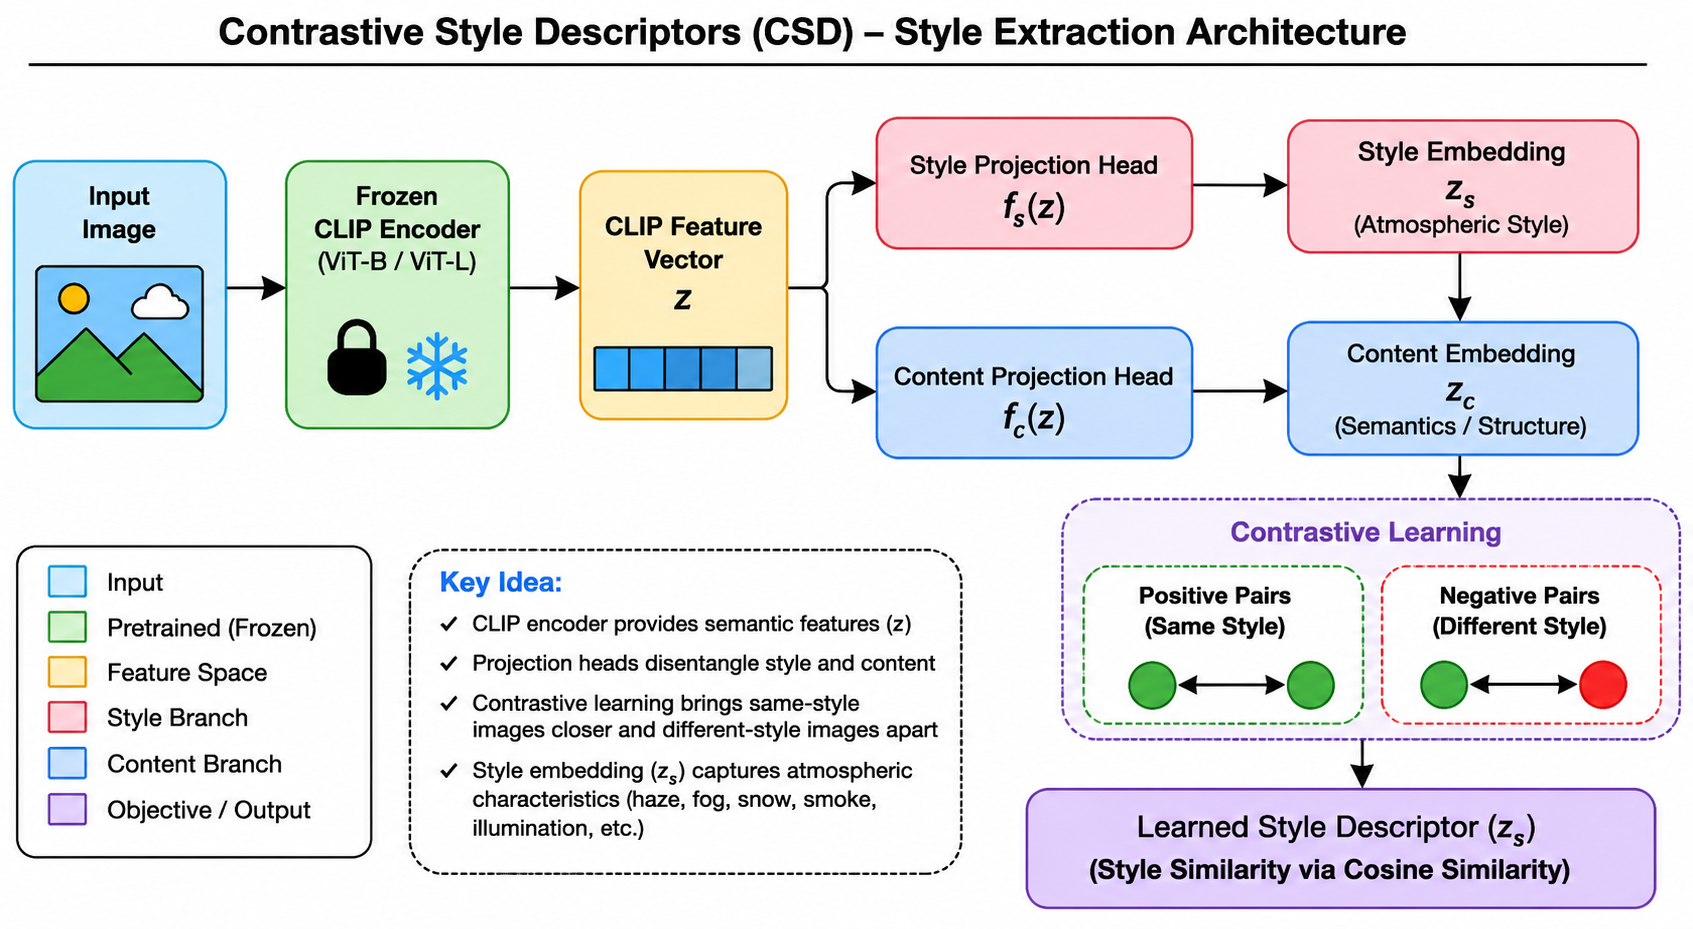
\includegraphics[width=0.85\linewidth]{images/CSD_Architecture.png}
    \caption{CSD architecture. A frozen CLIP encoder produces a shared representation $z$, projected by separate style ($f_s$) and content ($f_c$) heads trained with contrastive objectives. The disentangled style embedding yields the similarity $\mathrm{Sim}(x_g, x_r)$ used as a style-guidance signal during denoising.}
    \label{fig:csd_architecture}
\end{figure}

% =====================================================
\section{Adapters, Structural Guidance, and Prompt Fusion}
\label{sec:adapters_control}

Adapters add modular control to pretrained diffusion models without retraining the backbone.

\subsection{ControlNet}
\label{sec:controlnet}

Zhang et al.~\cite{zhang2023controlnet} introduced ControlNet, which adds a zero-initialised side network that processes structural cues (edges, depth, segmentation) and merges them back into the U-Net via additive connections.
The side network mirrors the U-Net encoder layers; zero initialisation ensures the model begins as an exact copy of the base diffusion system and gradually learns to incorporate external structure only when relevant, preventing training instability.
Multiple conditioning types can be fused simultaneously, enabling precise and interpretable spatial control.
InstantStyle-Plus (Chapter~\ref{chap:adaptive_proposed}) uses Tile ControlNet for spatial structure preservation during style transfer.

\begin{figure}[!htbp]
  \centering
  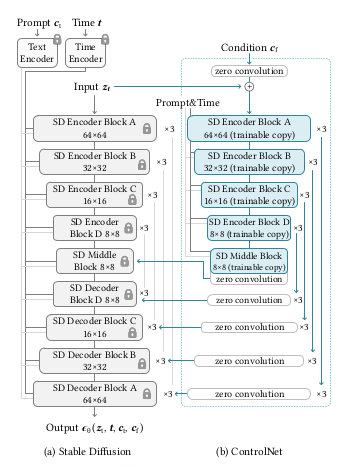
\includegraphics[width=0.7\linewidth]{images/controlnet_architecture.png}
  \caption{ControlNet: structure encoder merged into U-Net via additive connections (adapted from Zhang et al., 2023~\cite{zhang2023controlnet}).}
  \label{fig:controlnet_architecture}
\end{figure}
\FloatBarrier

\subsection{T2I-Adapter}
\label{sec:t2i_adapter}

Mou et al.~\cite{mou2024t2i} introduced T2I-Adapter, which provides lightweight structural conditioning through small adapter modules trained to align external guidance signals (sketch, depth, colour) with the internal feature space of a frozen text-to-image diffusion model.
Unlike ControlNet, T2I-Adapter uses a separate compact encoder rather than a full copy of the U-Net, significantly reducing the number of additional parameters while achieving comparable spatial controllability.

\subsection{IP-Adapter}
\label{sec:ip_adapter}

Ye et al.~\cite{ye2023ipadapterfidelityadapters} introduced IP-Adapter, which injects style from a reference image via decoupled cross-attention alongside text embeddings.
InstantStyle~\cite{wang2024instantstyle} demonstrated that style and spatial structure are not uniformly distributed across U-Net blocks --- \texttt{up\_blocks.0} and \texttt{up\_blocks.1} carry style information while remaining blocks carry layout and semantic content.
By restricting IP-Adapter injection to only these style blocks, InstantStyle achieves style injection without layout transfer.
InstantStyle-Plus~\cite{wang2024instantstyleplus} further extends this with Tile ControlNet for layout-preserving style transfer when a content image is available.
Text dictates \emph{what} to draw; the reference image defines \emph{how} it should appear --- controlling tone, colour, and texture without disturbing geometry.

\begin{figure}[!htbp]
  \centering
  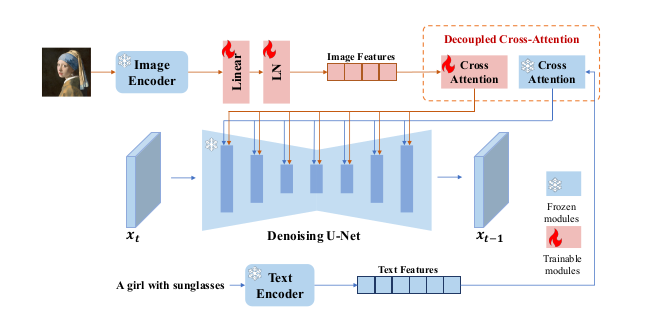
\includegraphics[width=0.7\linewidth]{images/ip_adapter_architecture.png}
  \caption{IP-Adapter: decoupled attention merges text semantics and image-based style cues (adapted from Ye et al., 2023~\cite{ye2023ipadapterfidelityadapters}).}
  \label{fig:ip_adapter_architecture}
\end{figure}
\FloatBarrier

% =====================================================
\section{Optimization-Guided Diffusion}
\label{sec:opt_guided_diffusion}

In a diffusion model, images are generated by iteratively denoising an image, gradually converting noise to structure.
Traditional diffusion models primarily use textual conditioning and cross-attention mechanisms, but recent studies have explored the direct incorporation of external objectives into the denoising trajectory.
These methods, referred to as optimization-guided diffusion, exploit additional guidance signals to steer the reverse diffusion process and direct generated samples towards desired properties.

\noindent Optimization-guided diffusion extends the controllability of diffusion models beyond standard prompt conditioning by using gradients from auxiliary objectives.
Such objectives can be class labels, semantic attributes, style descriptors, perceptual similarity measures, or task-specific constraints.
These approaches provide a flexible framework to control generation by modifying the denoising trajectory during sampling, without the need to retrain the model.

\subsection{Classifier Guidance}

One of the first approaches suggested for controllable diffusion generation was classifier guidance~\cite{dhariwal2021diffusion}.
The basic idea is to use an external classifier to provide gradients that help generated samples conform to a desired target class.
During reverse diffusion, the score estimate is modified with the gradient of the classifier log-probability:
\begin{equation}
    \nabla_{x_t} \log p(x_t \mid y) = \nabla_{x_t} \log p(x_t) + w\,\nabla_{x_t} \log p(y \mid x_t),
\end{equation}
where $y$ is the target condition, $w$ controls the strength of guidance, and $x_t$ is the noisy sample at timestep $t$.
Classifier guidance improves controllability and sample fidelity significantly, but requires training an additional classifier robust to noisy intermediate states, which increases computational complexity and limits practical usability.

\subsection{Classifier-Free Guidance (CFG)}

Classifier-Free Guidance trains conditional and unconditional diffusion models jointly to eliminate the need for an auxiliary classifier.
At inference time, the final score estimate is a combination of the conditional and unconditional predictions:
\begin{equation}
    \hat{\epsilon}_{\mathrm{CFG}} = \epsilon_{\mathrm{uncond}} + s\,\bigl(\epsilon_{\mathrm{cond}} - \epsilon_{\mathrm{uncond}}\bigr),
\end{equation}
where $s$ is the guidance scale.
In modern diffusion systems such as Stable Diffusion and SDXL~\cite{podell2023sdxlimprovinglatentdiffusion}, CFG has become the de-facto guidance mechanism.
The guidance scale can be adjusted to control the trade-off between prompt adherence and image diversity.

\subsection{Stable Diffusion with Constraints}

Recent work has explored embedding explicit constraints into diffusion sampling.
Constrained Stable Diffusion uses an optimization-based guidance to enforce desired properties during generation without additional model training.
The general constrained sampling problem is:
\begin{equation}
    \min_{x}\; f(x) \quad \text{subject to} \quad g(x) \le 0,
\end{equation}
where $f(x)$ is the diffusion objective and $g(x)$ is a user-defined constraint.
A projection and correction step during reverse diffusion produces a process that satisfies perceptual, semantic, or stylistic constraints, providing a principled approach to integrate external guidance signals while preserving the generative capabilities of the pretrained model.

\subsection{Langevin Dynamics}

Langevin dynamics is a stochastic optimization method commonly applied in Bayesian inference and probabilistic sampling.
It combines gradient-based updates with random perturbations, allowing samples to explore complex probability distributions while gradually moving toward regions of high probability.
The standard Langevin update is:
\begin{equation}
    x_{t+1} = x_t + \gamma_t\,\nabla \log p(x_t) + \sqrt{2\gamma_t}\,\epsilon_t, \qquad \epsilon_t \sim \mathcal{N}(0,I),
\end{equation}
where $\gamma_t$ is the step size.
The interplay between deterministic gradient ascent and stochastic exploration allows Langevin dynamics to escape poor local optima and converge to desired distributions.

\subsection{Proximal Langevin Dynamics}

Proximal Langevin Dynamics~\cite{zampini2025constrained} generalises classical Langevin sampling to optimization problems with explicit constraints or non-differentiable regularisation terms.
Instead of direct gradient updates, proximal operators project intermediate solutions onto feasible sets defined by the constraints:
\begin{equation}
    x_{t+1} = \mathrm{prox}_{\lambda g}\!\left(x_t + \gamma_t\,\nabla \log p(x_t) + \sqrt{2\gamma_t}\,\epsilon_t\right),
\end{equation}
where $\mathrm{prox}_{\lambda g}$ denotes the proximal operator of constraint function $g$.
This formulation provides a mathematically principled way to incorporate constraints into stochastic sampling procedures.
Chapter~\ref{chap:csd_style} evaluates this approach with CSD similarity as the constraint function; the trial experiments chapter applies it with AFNO style features.
In practice, gradient instability through the VAE decoder and sensitivity to the convergence threshold limit its scalability.

% =====================================================
\section{Physics-Based Atmospheric Image Formation}
\label{sec:atmospheric_physics}

Light interacting with particles suspended in the atmosphere creates atmospheric phenomena such as haze, fog, smoke, and dust.
These effects follow well-established physical processes --- scattering, absorption, and transmission --- unlike purely appearance-based image transformations.
Physics-based image formation models therefore provide a principled means of simulating atmospheric degradations and their impact on visual perception.

\subsection{Atmospheric Scattering Theory}

Some of the incident radiance is either scattered or absorbed by a participating medium before it reaches the camera as light propagates through it.
The extent of attenuation depends on particle density, viewing distance, and wavelength of light, leading to decreased visibility, contrast degradation, and colour shifts characteristic of adverse weather conditions.

\noindent Atmospheric image formation is commonly represented as the sum of two components: attenuated scene radiance and airlight.
The attenuated radiance is the light from scene objects that arrives at the camera after transmission through the atmosphere.
Airlight is the scattered environmental illumination accumulated along the viewing path.

\subsection{Koschmieder Model}

The Koschmieder model~\cite{koschmieder1924theorie} is one of the most commonly used models for atmospheric scattering and describes image formation under homogeneous atmospheric conditions.
The observed image intensity is:
\begin{equation}
    I(x) = J(x)\,T(x) + A\,\bigl(1-T(x)\bigr),
\end{equation}
where $I(x)$ is the observed image, $J(x)$ is the scene radiance, $A$ is the global atmospheric light, and $T(x)$ is the transmission map.
The transmission map is defined as:
\begin{equation}
    T(x) = e^{-\beta\, d(x)},
\end{equation}
where $\beta$ is the atmospheric extinction coefficient and $d(x)$ is the scene depth.
The model captures two major atmospheric effects: attenuation of scene radiance and accumulation of scattered atmospheric light.
As depth increases, transmission decreases, resulting in reduced visibility and stronger atmospheric effects.
The physics-grounded synthesis pipeline (Chapter~\ref{chap:phase2_pipeline}) uses the Koschmieder model as a depth-consistent compositor.

\begin{figure}[!htbp]
  \centering
  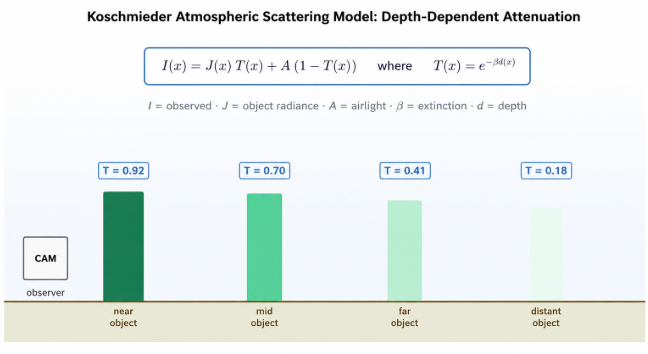
\includegraphics[width=0.92\linewidth]{images/figure_2.13.png}
  \caption{Schematic of atmospheric image formation with the Koschmieder scattering model: foreground objects appear clear while distant objects dissolve into the atmospheric medium.}
  \label{fig:koschmieder}
\end{figure}
\FloatBarrier

\subsection{Dark Channel Prior}

The Dark Channel Prior (DCP)~\cite{he2009dark} is a widely used technique for estimating atmospheric transmission from a single image.
The method is based on the observation that most natural outdoor images contain pixels with very low intensity values in at least one colour channel.
This property is exploited to estimate atmospheric light and transmission maps without requiring depth information.
Originally introduced for image dehazing, DCP has become an important tool for understanding atmospheric image formation and visibility degradation.
In the physics-grounded synthesis pipeline, the DCP is used to estimate per-domain $\beta$ and $A$ values from reference atmospheric photographs.

\subsection{Monocular Depth Estimation}

In atmospheric scattering models, depth is the main factor, as the degree of degradation is proportional to the distance of the object.
With recent progress in transformer-based depth estimation, accurate monocular depth estimation from a single RGB image is now feasible.
Methods such as MiDaS and DPT (Dense Prediction Transformers)~\cite{ranftl2021dpt} leverage large-scale pretraining and transformer architectures to predict dense depth maps across diverse environments.
These depth estimates can be combined with atmospheric scattering models to generate physically consistent, scene-geometry-dependent degradations.

\noindent By combining depth estimation and atmospheric scattering models, a physics-based framework for synthesising environmental effects is obtained.
In contrast to purely appearance-based stylisation approaches, depth-aware atmospheric formation explicitly models the attenuation of visibility and the degradation of the environment with respect to distance, enabling more realistic and controllable environmental transformations.
In the physics-grounded synthesis pipeline, DPT-Large depth maps drive the transmission map $T(x)$ computation for the Koschmieder compositor.

% =====================================================
\section*{Summary}

Research has steadily advanced toward controllable and interpretable generation.
Transformers introduced attention mechanisms; ViTs extended them to vision; GANs and VAEs pioneered generative modelling.
Diffusion unified these ideas into a stable probabilistic framework, enhanced by latent conditioning, cross-attention, and adapters such as ControlNet, T2I-Adapter, and IP-Adapter.
AFNO provides frequency-domain adaptation for frozen ViT backbones, enabling efficient correction for atmospheric distribution shifts.
Contrastive systems such as CLIP and CSD add semantic and stylistic grounding, while physics-based Koschmieder compositing provides the final layer of physical realism.
Together, these components form the complete methodological foundation of the work presented in the following chapters.
